\documentclass[12pt,a4paper]{report}

\usepackage{iftex}
\usepackage[a4paper,margin=2.5cm]{geometry}
\usepackage{graphicx}
\usepackage{array}
\usepackage{booktabs}
\usepackage{longtable}
\usepackage{tabularx}
\usepackage{multirow}
\usepackage{float}
\usepackage{caption}
\usepackage{setspace}
\usepackage{titlesec}
\usepackage{enumitem}
\usepackage{xcolor}
\usepackage{amsmath}
\usepackage{fancyhdr}
\usepackage{hyperref}
\usepackage[numbers,sort&compress]{natbib}

\ifPDFTeX
  \usepackage[utf8]{inputenc}
  \usepackage[T2A]{fontenc}
  \usepackage[english,russian]{babel}
\else
  \usepackage{fontspec}
  \setmainfont{FreeSerif}
  \setsansfont{DejaVu Sans}
  \setmonofont{DejaVu Sans Mono}
\fi

\hypersetup{
  unicode=true,
  colorlinks=true,
  linkcolor=black,
  citecolor=black,
  urlcolor=blue,
  pdftitle={SISI агентын завсрын тайлан},
  pdfauthor={Авиддарам Базаррагчаа}
}

\setstretch{1.25}
\setlength{\parindent}{1.25cm}
\setlength{\parskip}{0.2em}
\setlist[itemize]{leftmargin=2em}
\setlist[enumerate]{leftmargin=2em}
\captionsetup{font=small,labelfont=bf}

\titleformat{\chapter}[hang]{\bfseries\Large}{\thechapter.}{0.7em}{}
\titleformat{\section}[hang]{\bfseries\large}{\thesection}{0.7em}{}
\titleformat{\subsection}[hang]{\bfseries\normalsize}{\thesubsection}{0.7em}{}

\pagestyle{fancy}
\fancyhf{}
\fancyhead[R]{\thepage}
\fancyhead[L]{SISi системийн ухаалаг агент}
\renewcommand{\headrulewidth}{0.3pt}

\newcommand{\UniversityName}{Монгол Улсын Их Сургууль}
\newcommand{\SchoolName}{Мэдээллийн технологи, электроникийн сургууль}
\newcommand{\DepartmentName}{Мэдээлэл, компьютерын ухааны тэнхим}
\newcommand{\ProgramName}{Мэдээллийн систем}
\newcommand{\StudentName}{Авиддарам Базаррагчаа}
\newcommand{\StudentCode}{21B1NUM1186}
\newcommand{\AdvisorName}{О.Билгүүн}
\newcommand{\ReportTitle}{SISi системийн ухаалаг агент: оюутны порталд суурилсан хиймэл оюуны туслах системийн загварчлал ба завсрын хэрэгжилт}
\newcommand{\ReportTitleEn}{Intelligent Agent for the SISi System: Design and Midway Implementation of an AI Assistant for a Student Portal}
\newcommand{\ReportCity}{Улаанбаатар}
\newcommand{\ReportYear}{2026}

\begin{document}
\pagenumbering{gobble}

\begin{titlepage}
  \begin{center}
    {\large \UniversityName \par}
    \vspace{0.2cm}
    {\large \SchoolName \par}
    \vspace{0.2cm}
    {\large \DepartmentName \par}

    \vfill

    {\Large \StudentName \par}
    \vspace{1cm}

    {\bfseries\LARGE \ReportTitle \par}
    \vspace{0.6cm}
    {\large (\ReportTitleEn) \par}
    \vspace{0.8cm}

    {\large \ProgramName \par}
    \vspace{0.3cm}
    {\large Бакалаврын судалгааны ажлын завсрын тайлан \par}

    \vfill

    {\large \ReportCity \par}
    {\large \ReportYear\ оны хаврын улирал \par}
  \end{center}
\end{titlepage}

\begin{titlepage}
  \begin{center}
    {\large \UniversityName \par}
    \vspace{0.2cm}
    {\large \SchoolName \par}
    \vspace{0.2cm}
    {\large \DepartmentName \par}

    \vfill

    {\bfseries\LARGE \ReportTitle \par}
    \vspace{0.6cm}
    {\large \ProgramName \par}
    \vspace{0.4cm}
    {\large Бакалаврын судалгааны ажлын завсрын тайлан \par}

    \vfill

    \begin{tabular}{p{5cm}p{8cm}}
      Удирдагч: & \AdvisorName \\
      Гүйцэтгэсэн: & \StudentName\ (\StudentCode) \\
    \end{tabular}

    \vfill

    {\large \ReportCity \par}
    {\large \ReportYear\ оны 3 дугаар сар \par}
  \end{center}
\end{titlepage}

\cleardoublepage
\thispagestyle{empty}
\begin{center}
  {\Large Зохиогчийн баталгаа}
\end{center}
\vspace{0.8cm}

Миний бие \StudentName\ нь ``\ReportTitle'' сэдэвт бакалаврын судалгааны ажлын завсрын тайланг өөрийн гүйцэтгэсэн ажлын явц, одоогийн хэрэгжилт, цаашдын төлөвлөгөөнд тулгуурлан боловсруулснаа баталж байна. Энэхүү тайланд ашигласан эх сурвалж, онолын материал, системийн тайлбар, диаграмм болон үнэлгээний санааг холбогдох хэсгүүдэд дурдсан болно.

\vspace{1.4cm}
\noindent Гарын үсэг: \rule{6cm}{0.4pt}

\vspace{0.8cm}
\noindent Огноо: \rule{6cm}{0.4pt}

\cleardoublepage
\pagenumbering{roman}
\tableofcontents
\listoffigures
\listoftables

\cleardoublepage
\pagenumbering{arabic}
\setcounter{page}{1}

\chapter*{УДИРТГАЛ}
\addcontentsline{toc}{chapter}{УДИРТГАЛ}
Энэхүү тайлан SISi системийн ухаалаг агент төслийн судалгааны үр дүн, системийн шаардлага, архитектурын шийдэл болон одоогийн хэрэгжилтийн явцыг дүгнэн хүргэж байна. Төслийн зорилго нь SISI портал болон бусад холбогдох системүүдийн өгөгдлийг байгалийн хэлний интерфейсээр дамжуулан хэрэглэгчийн хүсэлтийг бодит үйлдэл болгон хувиргах хиймэл оюуны туслах систем бий болгоход оршино.

Одоогийн байдлаар төслийн хүрээнд Chrome extension-д суурилсан хэрэглэгчийн оролцоо, хиймэл оюуны сервер, SISI системийн API-г \textit{Model Context Protocol} (MCP) хэлбэрээр нэгтгэсэн локал интеграцын эхний хувилбар боловсруулагдаад байна. Мөн хуваарь, дүн, санхүү, мэдэгдэл, оюутны баримт бичгийн мэдээлэл зэрэг олон домэйнд зориулсан MCP хэрэгслүүд тодорхойлогдсон. Дараагийн шатанд бусад MCP серверүүдийг ерөнхий байдлаар холбох, Chrome extension-оор одоогийн сессийн access token-ийг дахин нэвтрэлт шаардахгүй ашиглах, багшийн порталын API-г нэмж Excel файлаас дүн оруулах ажиллагааг автоматжуулах зэрэг ажлууд үлдэж байна.

\chapter{ЗОРИЛГО}

Энэхүү бакалаврын судалгааны ажлын зорилго нь их сургуулийн SISI портал дээрх оюутанд хамаарах өгөгдөл, үйлчилгээг байгалийн хэлний интерфейсээр дамжуулан хүргэж, оюутны өдөр тутмын ажлыг хөнгөвчлөх хиймэл оюуны туслах системийн загварчлал, архитектур, эхний шатны хэрэгжилтийг боловсруулахад оршино.

Уг зорилгын хүрээнд систем нь оюутанд SISI портал дахь олон цэс, тархай мэдээллийг нэг цэгээс асууж авах боломж олгох, хичээлийн хуваарь, мэдэгдэл, дүн, санхүүгийн мэдээлэл зэрэг давтамж өндөртэй өгөгдөлд хурдан хүрэх замыг бүрдүүлэх, SISI болон цаашид холбогдох бусад MCP үйлчилгээний хооронд давтагддаг гар ажиллагааг бууруулах, мөн оюутны болон багшийн хүсэлтийг системийн бодит үйлдэлд холбох агентын суурь бий болгохыг зорьж байна.

\section{Зорилт}

Дээрх зорилгыг хэрэгжүүлэхийн тулд дараах зорилтуудыг дэвшүүлэв. Эхлээд оюутны портал ашиглах үед тулгардаг давтагддаг асуудал, хэрэгцээг тодорхойлох шаардлагатай. Үүний зэрэгцээ хиймэл оюуны агент, MCP, tool-calling загварын онолын үндсийг судалж, ижил төстэй боловсролын болон байгууллагын туслах системүүдийг харьцуулан үзэх нь чухал. Мөн SISi системийн ухаалаг агентын гол хэрэглэгчид, үндсэн ашиглалтын хувилбарууд, шаардлагуудыг тодорхойлох, системийн өндөр түвшний архитектур болон модулийн зохиомжийг боловсруулах, одоогийн кодын сан дээр тулгуурлан Chrome extension, AI сервер, локал MCP серверийн эхний хэрэгжилтийг баримтжуулах, access token-д суурилсан session reuse болон Chrome extension-ийн ашиглалтын загварыг тодорхойлох, цаашид хөгжүүлэх ерөнхий MCP өргөтгөлүүд, submit/export төрлийн функцүүд, мөн багшийн порталын Excel-д суурилсан дүн оруулах урсгалын төлөвлөгөөг гаргах зорилтуудыг дэвшүүлэв.

\chapter{СУДАЛГААНЫ ҮНДЭСЛЭЛ}

\section{Асуудлын тодорхойлолт}

Их сургуулийн оюутнууд өдөр бүр олон төрлийн академик мэдээлэлтэй харьцдаг. Хичээлийн хуваарь, шалгалтын хуваарь, дүн, кредит, төлбөрийн мэдээлэл, мэдэгдэл, баримт бичиг зэрэг өгөгдлүүд нь SISI порталын янз бүрийн цэс, дэд хуудсанд тархан байрладаг. Энэ нь хэрэглэгчийг нэг энгийн мэдээлэл авахын тулд олон товшилт хийх, хэд хэдэн дэлгэц дамжих шаардлагатай болгодог.

Жишээлбэл, оюутан ``маргаашийн хичээл хэдэн цагт эхлэх вэ'' гэсэн энгийн асуултад хариулахын тулд эхлээд порталд нэвтэрч, хуваарийн цэс рүү орж, тухайн өдрийн хичээлүүдийг олж, цагийг шалгах шаардлагатай. Үүнтэй адил ``миний GPA хэд вэ'', ``төлбөрийн үлдэгдэл хэд вэ'', ``дараагийн шалгалт хэзээ вэ'' зэрэг түгээмэл асуултууд бүгд олон алхам шаарддаг.

Энэ асуудал нь зөвхөн интерфейсийн төвөгтэй байдлаас үүдээгүй. Учир нь порталын архитектур нь өгөгдлийг функцээр нь салгасан бөгөөд хэрэглэгчийн ``зорилго''-ыг ойлгож өгдөг ухаалаг давхарга байхгүй. Одоогийн портал нь ``хуваарь харуулах'', ``дүн харуулах'' гэсэн тусдаа функцуудтай боловч ``миний энэ долоо хоногт хамгийн ачаалалтай өдөр аль вэ'' эсвэл ``миний сайжруулах шаардлагатай хичээлүүд юу вэ'' гэсэн илүү өндөр түвшний асуултад хариулах чадваргүй.

\section{Автоматжуулалтын хэрэгцээ}

Оюутнууд зөвхөн мэдээлэл уншаад зогсохгүй, уг мэдээллийг өөр системүүд рүү дамжуулах, боловсруулах хэрэгцээтэй байдаг. Тухайлбал, хичээлийн хуваариа Google Calendar-д оруулах, даалгаврын deadline-ийг todo app-д нэмэх, дүнгүүдийг Excel файл болгож хадгалах зэрэг ажлууд өдөр тутам давтагддаг. Эдгээр нь нэг бүрчлэн гүйцэтгэхэд хялбар боловч нийлээд ихээхэн цаг хугацаа, анхаарал шаарддаг.

Багш нарын хувьд ч мөн адил асуудал байдаг. Ялангуяа семестр бүрийн эцэст олон оюутны дүнг Excel файлаас системд гараар оруулах нь маш их цаг хугацаа шаардсан, алдаа гарах магадлал өндөр ажил юм. Нэг хичээлд 50-100 оюутан байх тохиолдолд энэ үйлдлийг автоматжуулах нь ихээхэн ач холбогдолтой.

\section{Хиймэл оюуны одоогийн чадамж ба хязгаарлалт}

Сүүлийн жилүүдэд хэлний загварууд (Large Language Models) гайхалтай хурдацтай хөгжиж, текст ойлгох, боловсруулах, үүсгэх чадварын хувьд хүний түвшинд хүрсэн байна. GPT-4, Claude, Gemini зэрэг загварууд нь нарийн төвөгтэй асуултад хариулах, код бичих, баримт бичиг боловсруулах, шинжилгээ хийх зэрэг даалгаврыг өндөр чанартай гүйцэтгэж чаддаг.

Гэсэн хэдий ч эдгээр загварууд нь ``хаалттай орчин''-д ажилладаг. Тэдгээр нь сургалтын үеийн мэдлэг дээр тулгуурлан хариулт үүсгэдэг бөгөөд бодит цагийн өгөгдөлд хандах, гаднах системтэй харилцах, хэрэглэгчийн өмнөөс үйлдэл гүйцэтгэх чадваргүй. Өөрөөр хэлбэл, загварын ``оюун ухаан'' хангалттай боловч бодит ертөнцтэй харилцах ``гар, хөл'' нь дутагдалтай.

Энэ хязгаарлалтыг шийдэх хамгийн үр дүнтэй арга нь загварын оюун ухааныг нэмэгдүүлэх бус, түүнд зохих хэрэгслүүдийг олгох явдал юм. Загварын параметрийн тоог нэмэгдүүлэх, илүү их өгөгдөл дээр сургах зэрэг incremental сайжруулалтаас илүүтэйгээр, загварт бодит системүүдтэй харилцах интерфейс хангах нь шинэ түвшний чадамж нээж өгдөг.

\section{Хувийн сэдэлт}

Энэхүү төслийг хэрэгжүүлэх хувийн сэдэлт нь дээрх онолын үндэслэлээс гадна практик туршлагаас үүдэлтэй. Би өөрөө NUM-ийн оюутан болохын хувьд SISI порталыг өдөр тутам ашигладаг бөгөөд түүний давуу болон сул талуудыг сайн мэддэг. Энэ нь надад бодит хэрэгцээнд тулгуурласан систем загварчлах, хөгжүүлэх боломжийг олгож байна.

Үүнээс гадна хиймэл оюуны загварт хэрэгсэл олгох (tool-use) чиглэлийг гүнзгий судлах, туршиж үзэх хүсэлтэй байсан. Загварын суурь оюун ухаан нь аль хэдийн хангалттай түвшинд хүрсэн бөгөөд түүнд зөв хэрэгслүүдийг олгосноор бодит амьдрал дээр нөлөө үзүүлэх систем бүтээх боломжтой гэдэгт итгэдэг. Энэхүү итгэл үнэмшлийг өөрт ойр, сайн мэддэг системээр туршиж баталгаажуулах нь энэ төслийн нэг зорилго юм.

\section{Асуудлын томьёолол}

Дээрх үндэслэлд тулгуурлан энэхүү судалгааны асуудлыг дараах байдлаар томьёолж байна: SISI портал болон холбогдох бусад системүүдийн өгөгдөл, үйлчилгээг найдвартай, аюулгүй, өргөтгөх боломжтой хэлбэрээр байгалийн хэлний интерфейстэй хэрхэн холбож, хэрэглэгчийн хүсэлтийг бодит системийн үйлдэл болгон хөрвүүлэх вэ?

Энэ асуудлыг шийдэхэд зөвхөн хэлний интерфейсийн өнгөц давхарга хангалтгүй. Систем нь бодит цагийн өгөгдөл ашиглах, хэрэглэгчийг дахин нэвтрүүлэхгүйгээр одоогийн сессийг аюулгүй ашиглах, унших үйлдэл болон бичих үйлдлийг ялгаж удирдах, олон системийн хооронд уялдаа хангах, мөн оюутны болон багшийн өөр өөр хэрэглээний хувилбарт тохирох модульчлагдсан бүтэцтэй байх шаардлагатай.

Иймээс энэхүү дипломын ажлын судалгааны гол чиглэл нь агентын онол, Model Context Protocol стандартыг ашигласан архитектур, мөн бодит интеграцын түвшний системийн загварчлал болно.

\chapter{ОНОЛЫН БОЛОН ХАРЬЦУУЛСАН СУДАЛГАА}

\section{Хиймэл оюуны агентын ойлголт}

Хиймэл оюуны агент гэдэг нь орчноо хүлээн авч, түүн дээр үндэслэн шийдвэр гаргаж, үйлдэл хийх чадвартай систем юм \citep{russell-norvig}. Сүүлийн үеийн хэлний загваруудын хувьд энэ ойлголт нь шинэ утга агуулгатай болсон. Загвар нь зөвхөн текст үүсгээд зогсохгүй, гаднах системүүдтэй харилцах хэрэгслүүдийг дуудаж, олж авсан мэдээллийг нэгтгэн, цаашдын үйлдлийг төлөвлөх чадвартай болсон.

Орчин үеийн AI агент нь гурван үндсэн бүрэлдэхүүнээс бүрдэнэ. Нэгдүгээрт, хэлний загвар (LLM) нь хэрэглэгчийн хүсэлтийг ойлгох, хариулт үүсгэх, шийдвэр гаргах ``тархи'' болж үйлчилнэ. Хоёрдугаарт, хэрэгслүүд (tools) нь загварт гаднах системүүдтэй харилцах боломжийг олгодог ``гар, хөл'' юм. Гуравдугаарт, orchestration давхарга нь хэрэгслүүдийг зөв дарааллаар дуудах, үр дүнг нэгтгэх, алдаа засах үүрэгтэй.

\subsection{ReAct загвар}

AI агентын нэг түгээмэл архитектур нь ReAct (Reasoning and Acting) загвар юм \citep{react-paper}. Энэ загварын гол санаа нь загварыг ``бодолт'' болон ``үйлдэл''-ийг ээлжлэн хийхэд сургах явдал. Загвар нь эхлээд асуудлыг задлан шинжилж (reasoning), дараа нь шаардлагатай хэрэгслийг дуудаж (acting), хэрэгслийн хариуг авч дахин бодолт хийж, эцсийн хариулт бүрдүүлдэг.

Энэ загвар нь хэрэглэгчийн хүсэлтийг шууд нэг хэрэгсэлд холбохоос илүү уян хатан юм. Жишээлбэл, ``миний хамгийн сул дүнтэй хичээл юу вэ'' гэсэн асуулт нь эхлээд дүнгийн жагсаалтыг авах, дараа нь хамгийн багыг нь олох гэсэн хоёр алхамыг агуулж байна. ReAct загвар нь ийм олон алхамт асуултыг шат дараатай шийдвэрлэх боломжийг олгодог.

\subsection{Tool-calling механизм}

Орчин үеийн хэлний загварууд нь tool-calling буюу функц дуудах чадвартай болсон \citep{openai-functions}. Энэ нь загварт тодорхой схемтэй хэрэгслүүдийн жагсаалт өгөх, загвар хэрэглэгчийн хүсэлтэд тохирох хэрэгслийг сонгож дуудах, хэрэгслийн хариуг загварт буцааж өгч эцсийн хариулт үүсгэхийг хэлнэ.

Tool-calling нь AI системийг ``хаалттай'' байдлаас ``нээлттэй'' байдалд шилжүүлдэг. Загвар нь өөрийн сургалтын өгөгдөлд хязгаарлагдахгүй, бодит цагийн өгөгдөлд хандах, гаднах системүүдтэй харилцах боломжтой болдог. Гэхдээ энэ нь мөн аюулгүй байдлын шинэ асуудлуудыг бий болгодог тул read-only болон mutation хэрэгслүүдийг ялгах, баталгаажуулалтын механизм нэмэх зэрэг арга хэмжээ шаардлагатай.

\section{Model Context Protocol (MCP)}

Model Context Protocol нь Anthropic компаниас санаачилсан нээлттэй стандарт бөгөөд хэлний загварт гадаад хэрэгсэл, өгөгдлийн эх үүсвэрийг стандартчилсан аргаар холбох зориулалттай \citep{mcp-intro}. MCP-ийн гол зорилго нь интеграцын ``N x M'' асуудлыг шийдвэрлэх явдал юм. Өөрөөр хэлбэл, N тооны AI application болон M тооны гаднах системийг нэг бүрчлэн холбохын оронд, нийтлэг протокол ашиглан хоёр талаас нэг удаа хэрэгжүүлэхэд хангалттай болгох.

\subsection{MCP-ийн бүтэц}

MCP нь гурван үндсэн нэгжтэй. Tools нь загвараас дуудагдах функцууд бөгөөд тодорхой үйлдэл гүйцэтгэж үр дүн буцаадаг. Resources нь загварт өгөгдөл, контекст хангах файл, өгөгдлийн эх үүсвэрүүд юм. Prompts нь загварт заавар, загвар өгөх урьдчилан бэлтгэсэн текстүүд юм.

MCP сервер нь эдгээр нэгжүүдийг ил гаргадаг бие даасан процесс бөгөөд MCP client нь тэдгээрийг ашигладаг AI application юм. Энэ хоёр тал нь JSON-RPC протоколоор харилцана.

\subsection{Энэхүү төсөлд MCP сонгосон шалтгаан}

SISi Intelligent Agent төсөлд MCP сонгох хэд хэдэн шалтгаан байв. Нэгдүгээрт, стандарт интерфейс нь SISI, багшийн портал, календарь, баримт боловсруулах үйлчилгээ зэрэг өөр өөр системийг ижил загвараар илэрхийлэх боломжийг олгодог. Хоёрдугаарт, модульчлагдсан бүтэц нь порталтай холбогдох логик, Chrome extension-д суурилсан хэрэглэгчийн оролт, ирээдүйн интеграцуудыг тусдаа давхаргад хөгжүүлэх боломжтой болгодог. Гуравдугаарт, өргөтгөх боломж нь шинэ хэрэгсэл нэмэхэд бүх системийг дахин бичих шаардлагагүй болгодог. Дөрөвдүгээрт, аюулгүй байдлын удирдлага нь read-only болон mutation хэрэгслүүдийг тусад нь загварчлах боломжтой.

\section{Ижил төстэй системүүдийн судалгаа}

AI туслах системүүдийн өнөөгийн байдлыг гурван чиглэлээр авч үзэв: боловсролын AI туслахууд, tool-use AI системүүд, байгууллагын автоматжуулалтын шийдлүүд.

\subsection{Боловсролын AI туслахууд}

Боловсролын салбарт хиймэл оюуныг ашигласан хэд хэдэн систем байна. Duolingo-ийн AI туслах нь хэл сурахад харилцан ярилцах, алдаа засах, тайлбар өгөх чадвартай. Carnegie Learning-ийн MATHia платформ нь математикийн даалгавар шийдэхэд алхам алхмаар туслах, оюутны ахицыг хянах боломжтой \citep{carnegie-learning}. IBM Watson Education нь сургалтын материалыг хувь хүнд тохируулах, асуултад хариулах зэрэг функцтэй.

Эдгээр системүүдийн нийтлэг шинж нь сургалтын агуулгад төвлөрсөн байдал юм. Тэд хичээл заах, тайлбар өгөх, дасгал шалгах зэрэгт чадварлаг боловч сургуулийн дотоод порталын өгөгдөл, хэрэглэгчийн хувийн академик мэдээлэлтэй гүн интеграц хийх зорилгогүй. Энэ нь SISi Intelligent Agent-аас ялгаатай бөгөөд тус төсөл нь нийтлэг сургалтын агуулга бус, тухайн оюутны бодит өгөгдөлд суурилдаг.

\subsection{Tool-use AI системүүд}

Tool-calling чадвар бүхий AI системүүд сүүлийн жилүүдэд хурдацтай хөгжиж байна. OpenAI-ийн GPT Actions нь гуравдагч талын API-уудтай холбогдох боломжийг олгодог бөгөөд хэрэглэгч өөрийн хэрэгцээнд тохируулсан интеграц хийх боломжтой \citep{openai-actions}. Anthropic-ийн Claude нь MCP-ээр дамжуулан файл систем, өгөгдлийн сан, вэб хөтөч зэрэгтэй харилцах чадвартай болсон. GitHub Copilot нь код бичих, засахаас гадна terminal команд ажиллуулах, файл удирдах боломжтой болж байна.

Эдгээр системүүд нь ерөнхий зориулалттай бөгөөд олон төрлийн даалгаварт ашиглагдах боломжтой. Гэхдээ тэд тодорхой нэг домэйнд (жишээлбэл их сургуулийн портал) зориулсан биш тул тухайн домэйны нарийн шаардлагууд, workflow-уудыг бүрэн хангахгүй.

\subsection{Байгууллагын автоматжуулалтын системүүд}

Байгууллагын хэмжээнд ашиглагддаг AI туслах системүүд ч бас холбогдох судалгааны объект болно. Intercom Fin нь хэрэглэгчийн асуултад автоматаар хариулах, шаардлагатай үед хүн рүү шилжүүлэх чадвартай \citep{intercom-fin}. Zendesk AI нь support ticket-үүдийг ангилах, хариулт санал болгох, нийтлэг асуултад автоматаар хариулах боломжтой. ServiceNow Virtual Agent нь байгууллагын дотоод системүүдтэй холбогдож, ажилчдын хүсэлтийг автоматаар шийдвэрлэх чадвартай.

Эдгээр системүүд нь байгууллагын дотоод өгөгдөлтэй холбогдох чадвараараа SISi Intelligent Agent-тай төстэй. Гэхдээ тэд ихэвчлэн худалдааны бүтээгдэхүүн бөгөөд тухайн байгууллагын нарийн хэрэгцээнд тохируулахад хязгаарлалттай байдаг.

\subsection{Харьцуулалтын дүгнэлт}

\begin{table}[H]
  \centering
  \caption{Ижил төстэй системүүдийн харьцуулалт}
  \label{tab:similar-systems}
  \begin{tabularx}{\textwidth}{>{\raggedright\arraybackslash}p{3cm} >{\raggedright\arraybackslash}X >{\raggedright\arraybackslash}X}
    \toprule
    Системийн төрөл & Давуу тал & SISi Intelligent Agent-тай харьцуулахад \\
    \midrule
    Боловсролын AI (Duolingo, Carnegie Learning) & Сургалтын агуулгад чадварлаг, харилцан яриа сайн & Оюутны хувийн академик өгөгдөл, порталын интеграц байхгүй \\
    \addlinespace
    Tool-use AI (GPT Actions, Claude MCP) & Олон төрлийн системтэй холбогдох ерөнхий чадвар & Тодорхой домэйнд зориулсан биш, их сургуулийн portal workflow мэдэхгүй \\
    \addlinespace
    Байгууллагын AI (Intercom, ServiceNow) & Дотоод системтэй холбогдох, автоматжуулалт & Худалдааны бүтээгдэхүүн, тохируулах боломж хязгаарлагдмал \\
    \addlinespace
    SISi Intelligent Agent & NUM-ийн SISI порталд зориулсан, MCP-д суурилсан модульчлагдсан архитектур & Одоогоор хөгжүүлэлтийн шатанд, бүрэн туршилт хийгдээгүй \\
    \bottomrule
  \end{tabularx}
\end{table}

Энэхүү харьцуулалтаас харахад зах зээл дээрх системүүд тус бүрдээ давуу талтай боловч NUM-ийн SISI порталын нарийн шаардлагууд, оюутны өдөр тутмын workflow-уудад зориулсан систем байхгүй байна. Энэ нь SISi Intelligent Agent төслийн шинэлэг тал бөгөөд тодорхой домэйнд зориулсан AI агентыг MCP стандартаар загварчилсан нь бусад системээс ялгаатай онцлог болно.

\section{Судалгааны дүгнэлт}

Онолын болон харьцуулсан судалгааны үр дүнд хэд хэдэн дүгнэлтэд хүрэв.

Нэгдүгээрт, SISi Intelligent Agent төрлийн системд дан ганц LLM хангалтгүй бөгөөд бодит системтэй холбогдох агент архитектур шаардлагатай. Загварын оюун ухаан хангалттай боловч түүнд зохих хэрэгслүүдийг олгох шаардлагатай.

Хоёрдугаарт, Model Context Protocol нь тус төслийн хувьд интеграцын давхаргыг стандартчилах, өргөтгөх, аюулгүй удирдах хамгийн тохиромжтой шийдлийн нэг юм. MCP нь олон системийг нэг протоколоор холбох, read-only болон mutation хэрэгслүүдийг ялгах боломжийг олгодог.

Гуравдугаарт, ижил төстэй системүүд байдаг боловч NUM-ийн SISI порталын хэрэглээ, өгөгдөл, workflow-д чиглэсэн тусгай шийдэл хэрэгтэй. Ерөнхий зориулалтын tool-use AI системүүд нь энэ хэрэгцээг бүрэн хангахгүй.

Дөрөвдүгээрт, судалгааны дараагийн гол алхам нь архитектурын зөв сонголтыг бодит хэрэгжилт болон хэрэглэгчийн үнэлгээгээр баталгаажуулах явдал юм.

\chapter{СИСТЕМИЙН ШИНЖИЛГЭЭ}

\section{Оролцогч талууд}

Энэхүү системийн үндсэн хэрэглэгч нь оюутан боловч системийн бүрэн хэрэглээнд багш, удирдагч, сургуулийн системийн администратор, мөн MCP-ээр холбогдох бусад системийн орчин нөлөөлнө.

Оюутан нь системийн гол хэрэглэгч бөгөөд хуваарь, дүн, мэдэгдэл, баримт бичиг, даалгаврын мэдээллийг хурдан авах, дахин нэвтрэлтгүйгээр өдөр тутмын ажлаа автоматжуулах сонирхолтой. Багш нь багшийн порталтай холбогдсон үед дүн оруулах, ялангуяа Excel файлаас олон оюутны дүнг хялбар оруулах зэрэг ажлыг автоматжуулахыг хүсдэг. Удирдагч багш болон комисс нь системийн судалгааны үндэслэл, архитектурын зөв байдал, хэрэгжих боломж, ахицыг үнэлэх үүрэгтэй. Сургуулийн системийн орчин нь порталын нэвтрэлт, API өөрчлөлт, өгөгдлийн бодит байдал, аюулгүй байдлын шаардлагыг тодорхойлно. Бусад MCP үйлчилгээнүүд нь ирээдүйд холбогдох календарь, баримт бичиг, өгөгдөл экспорт, бусад автоматжуулалтын интеграцын боломжийг бүрдүүлнэ.

\section{Ашиглалтын хувилбарууд}

Системийн гол ашиглалтын хувилбаруудыг Зураг~\ref{fig:usecases}-д нэгтгэн үзүүлэв. Эдгээр use case-үүдийг одоогийн хэрэгжилтийн төлөвийн хамт Хүснэгт~\ref{tab:usecases}-д тайлбарлав.

\begin{figure}[H]
  \centering
  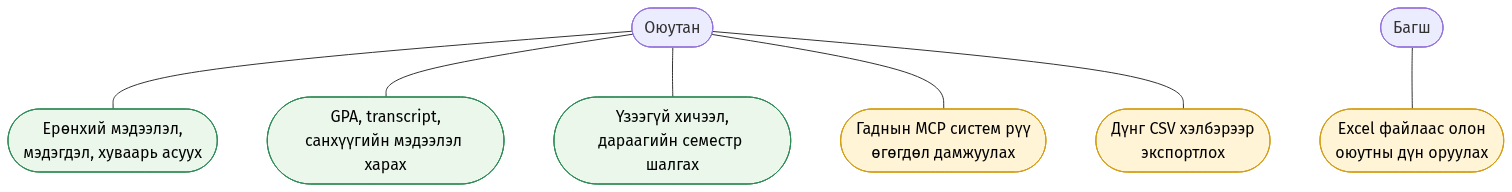
\includegraphics[width=0.95\textwidth]{assets/diagrams/usecases.png}
  \caption{SISi Intelligent Agent-ын үндсэн ашиглалтын хувилбарууд}
  \label{fig:usecases}
\end{figure}

% ШИНЭ ДИАГРАМ ХЭРЭГТЭЙ: Use case диаграмыг шинэчлэх. Оюутан болон Багш гэсэн хоёр actor-той, 
% UC-1-ээс UC-8 хүртэлх use case-үүдийг харуулсан UML use case диаграм.
% Оюутан: UC-1 (Ерөнхий мэдээлэл), UC-2 (Хуваарь), UC-3 (Дүн/GPA), UC-4 (E-journal), 
%         UC-5 (MCP интеграц), UC-6 (CSV export)
% Багш: UC-7 (Excel-ээс дүн оруулах), UC-8 (Баталгаажуулалт)
% Нийтлэг: Session bootstrap

\begin{table}[H]
  \centering
  \caption{Үндсэн use case-үүд ба тэдгээрийн төлөв}
  \label{tab:usecases}
  \begin{tabularx}{\textwidth}{>{\raggedright\arraybackslash}p{1cm} >{\raggedright\arraybackslash}X >{\raggedright\arraybackslash}p{3cm}}
    \toprule
    № & Тодорхойлолт & Төлөв \\
    \midrule
    UC-1 & Оюутны ерөнхий мэдээлэл, идэвхтэй хичээлүүд, порталын мэдэгдлийг байгалийн хэлээр асууж авах & MCP tool бэлэн \\
    UC-2 & Хичээлийн болон шалгалтын хуваарийг асууж авах, тодорхой өдөр эсвэл долоо хоногоор шүүх & MCP tool бэлэн \\
    UC-3 & Дүн, GPA, transcript, кредитийн мэдээллийг харах, шинжлэх & MCP tool бэлэн \\
    UC-4 & E-journal-ийн мэдээлэл, үнэлгээний бүрэлдэхүүн хэсгүүдийг харах & Хэсэгчлэн бэлэн \\
    UC-5 & Порталын өгөгдлийг MCP-ээр холбогдсон гаднын системүүд рүү (календарь, todo app) дамжуулах & Төлөвлөсөн \\
    UC-6 & Дүн, хуваарь зэрэг өгөгдлийг CSV эсвэл бусад форматаар экспортлох & Төлөвлөсөн \\
    UC-7 & Багшийн порталын API ашиглан Excel файлаас олон оюутны дүн оруулах & Төлөвлөсөн \\
    UC-8 & Эрсдэлтэй үйлдэл (mutation) хийхээс өмнө хэрэглэгчээс баталгаажуулалт авах & Төлөвлөсөн \\
    \bottomrule
  \end{tabularx}
\end{table}

UC-1-ээс UC-3 хүртэлх use case-үүд нь MCP серверт бүрэн хэрэгжсэн бөгөөд SISI API-гаас оюутны үндсэн мэдээлэл, хуваарь, дүн, санхүүгийн мэдээллийг амжилттай уншиж байна. UC-4 нь e-journal хэсгийн зарим API хязгаарлалтаас болж хэсэгчлэн хэрэгжсэн. UC-5-аас UC-8 хүртэлх use case-үүд нь дараагийн шатанд хэрэгжих төлөвлөгөөтэй.

\section{Функциональ шаардлага}

Системийн функциональ шаардлагыг дараах байдлаар тодорхойлов.

\subsection{Хэрэглэгчийн оролт ба гаралт}

Хэрэглэгч Chrome extension-оор дамжуулан байгалийн хэлээр асуулт, даалгавар өгөх боломжтой байх ёстой. Систем нь хэрэглэгчийн хүсэлтийг ойлгож, шаардлагатай мэдээллийг цуглуулж, ойлгомжтой текст хэлбэрээр хариулах чадвартай байна. Хариулт нь зөвхөн түүхий өгөгдөл бус, хэрэглэгчид ойлгомжтой тайлбар, дүгнэлт агуулсан байх ёстой.

\subsection{Өгөгдөлд хандалт}

Систем нь оюутны идэвхтэй сесс дээр тулгуурлан SISI API-гаас бодит өгөгдөл унших чадвартай байна. Хэрэглэгчийг дахин нэвтрүүлэхгүйгээр тухайн порталаас авсан access token эсвэл холбогдох сессийн мэдээллийг аюулгүй бүртгэдэг байх шаардлагатай. Хуваарь, дүн, санхүү, мэдэгдэл, баримт бичиг, e-journal зэрэг үндсэн домэйнүүдийг тусдаа MCP хэрэгслээр дуудах боломжтой байна.

\subsection{Өргөтгөх чадвар}

Систем нь ирээдүйд дурын MCP нийцтэй гаднын үйлчилгээ болон багшийн порталын API-тай холбогдох өргөтгөх чадвартай байх ёстой. Шинэ хэрэгсэл нэмэхэд бүх системийг дахин бичих шаардлагагүй байх модульчлагдсан бүтэцтэй байна.

\subsection{Аюулгүй байдал}

Экспорт, submit зэрэг mutation үйлдэлд хэрэглэгчээс баталгаажуулалт шаардах механизмтай байна. Хэрэглэгчийн session-id, хугацаа дуусах төлөв, зөвшөөрөгдсөн origin-уудыг удирдах чадвартай байх шаардлагатай. Read-only болон mutation хэрэгслүүдийг тодорхой ялгаж, mutation-д нэмэлт хяналт тавина.

\section{Функциональ бус шаардлага}

\subsection{Аюулгүй байдал}

Систем нь нэвтрэх мэдээллийг ил хадгалахгүй байх ёстой. Локал сессийн хугацааг хязгаарлаж (idle TTL), зөвшөөрөгдсөн origin ашиглах замаар аюулгүй байдлыг хангана. Access token болон cookie-г AI загварт шууд ил гаргахгүй, зөвхөн MCP серверээр дамжуулан хэрэглэнэ.

\subsection{Өргөтгөх чадвар}

Шинэ MCP домэйн, шинэ гадаад интеграц, шинэ client төрлүүдийг бага өөрчлөлтөөр нэмэх боломжтой байна. Модульчлагдсан архитектур нь бүрэлдэхүүн хэсгүүдийг бие даан хөгжүүлэх, туршихад тохиромжтой.

\subsection{Найдвартай байдал}

Upstream API алдаа гарсан тохиолдолд систем нь ойлгомжтой алдааны мэдэгдэл буцаах ёстой. Хэрэглэгчид юу болсныг мэдэгдэж, шаардлагатай бол дахин оролдох боломж олгоно.

\subsection{Гүйцэтгэл}

Энгийн унших хүсэлтүүдийг боломжит богино хугацаанд гүйцэтгэх ёстой. MCP серверийн хариу хугацаа нь upstream API-ийн хариу хугацаанаас хамаарах боловч нэмэлт саатал хамгийн бага байх ёстой.

\subsection{Хянах боломж}

Аль хэрэгсэл ямар өгөгдөл ашигласныг тайлбарлах боломжтой байна. Mutation үйлдлүүдийн түүх, лог бичлэг хадгалагдах ёстой.

\subsection{Хэрэглэх боломж}

Порталд аль хэдийн нэвтэрсэн хэрэглэгч нэмэлт нэвтрэлтгүйгээр системийг ашиглахад ойлгомжтой байх ёстой. Байгалийн хэлний интерфейс нь техникийн мэдлэг шаардахгүй, энгийн хүмүүст хүртээмжтэй байна.

\section{Эрсдэл ба хязгаарлалт}

Завсрын шатанд хэд хэдэн эрсдэл, хязгаарлалт ажиглагдаж байна.

SISI порталын API нь албан ёсны тогтвортой public contract биш байж болох тул ирээдүйд өөрчлөлт гарч болзошгүй. Энэ тохиолдолд MCP серверийн upstream client-ийг шинэчлэх шаардлагатай болно. Гэхдээ модульчлагдсан архитектур нь энэ өөрчлөлтийг бусад бүрэлдэхүүнүүдэд нөлөөлөхгүйгээр хийх боломжийг олгоно.

Бичих үйлдэлтэй холбоотой submit, export, state change төрлийн функцуудыг шууд нээх нь аюулгүй байдлын нэмэлт шалгалт шаарддаг. Буруу хэрэглэгч эсвэл буруу ойлгосон команд нь санамсаргүй өөрчлөлт хийх эрсдэлтэй тул баталгаажуулалтын давхарга заавал хэрэгтэй.

Хиймэл оюуны загварын тайлбарлал буруу байвал буруу хэрэгсэл дуудах эрсдэлтэй. Жишээлбэл, ``миний дүн'' гэж асуухад санхүүгийн дүн буцаах зэрэг алдаа гарч болно. Иймд tool routing-ийн логик, хэрэгслийн тодорхойлолт, загварын prompt зэргийг сайтар загварчлах шаардлагатай.

Олон төрлийн MCP үйлчилгээ болон багшийн порталын mutation урсгал нэмэгдэхэд зөвшөөрөл, аудит, алдаа шалгалтын төвөгшил өсөх болно. Энэ нь архитектурын цэвэр байдал, баримт бичгийн чанар, туршилтын хамрах хүрээг улам чухал болгоно.

\chapter{СИСТЕМИЙН ЗОХИОМЖ}

\section{Ерөнхий архитектур}

Системийн ерөнхий архитектурыг Зураг~\ref{fig:architecture}--д үзүүлэв. Архитектур нь дөрвөн үндсэн давхаргатай: Chrome extension-д суурилсан хэрэглэгчийн оролтын давхарга, хэлний загвар болон хариултын урсгалыг удирдах AI сервер, SISI API-г MCP хэлбэрт оруулсан локал интеграцын давхарга, SISI, багшийн портал, цаашдын бусад MCP үйлчилгээ зэрэг гаднын системүүд.

\begin{figure}[H]
  \centering
  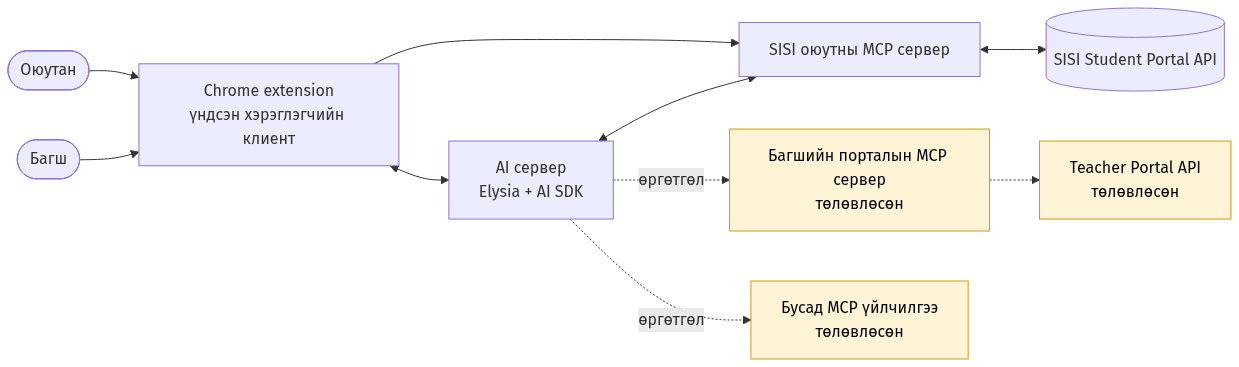
\includegraphics[width=\textwidth]{assets/diagrams/architecture.png}
  \caption{SISi системийн ухаалаг агентын өндөр түвшний архитектур}
  \label{fig:architecture}
\end{figure}

Энэхүү архитектурын гол давуу тал нь Chrome extension, AI сервер, порталын интеграцын давхаргуудыг тусгаарлаж өгсөнд оршино. Ингэснээр хэрэглэгчийн клиент, загвар, MCP серверүүд, read-only болон mutation үйлдлийг бие даан хөгжүүлэх боломж бүрдэнь.

\section{Модулийн зохиомж}

Одоогийн кодын сан дээрх хэрэгжилтийг модульчлан авч үзвэл Хүснэгт~\ref{tab:modules} дахь бүтэцтэй байна.

\begin{table}[H]
  \centering
  \caption{Одоогийн төслийн модулиуд}
  \label{tab:modules}
  \begin{tabularx}{\textwidth}{>{\raggedright\arraybackslash}p{3.4cm} >{\raggedright\arraybackslash}X}
    \toprule
    Модуль & Үүрэг \\
    \midrule
    \texttt{apps/web} & Туршилтын зориулалттай интерфейсийн суурь. Одоогийн зорилтот хэрэглээний үндсэн клиент биш боловч прототип туршихад ашиглагдаж болно. \\
    \texttt{apps/server} & Elysia дээрх AI сервер. Хэлний загвар, message урсгал, цаашдын MCP tool orchestration-ийг удирдах төв давхарга. \\
    \texttt{packages/mcp} & Локал MCP сервер. SISI API-тай холбогдож overview, schedule, academic, financial, notifications, student resources, top menus, e-journal зэрэг хэрэгслийг өгнө. \\
    \texttt{apps/extension} & Chrome extension-ийн үндсэн клиент. Порталын орчноос access token авч, хэрэглэгчийг дахин нэвтрүүлэхгүй session bootstrap хийх зорилготой. \\
    \texttt{packages/db} & Ирээдүйн лог, аудит, үнэлгээний өгөгдөл, mutation үйлдлийн мөрдөх боломжийг хадгалах давхарга. \\
    \bottomrule
  \end{tabularx}
\end{table}

\section{Сесс болон өгөгдлийн урсгал}

SISI API-д хандахын тулд хэрэглэгчийн хүчинтэй сесс шаардлагатай. Иймээс локал MCP сервер нь session register, refresh, clear гэсэн тусдаа endpoint-уудтай бөгөөд эхлээд хэрэглэгчийн сессийг баталгаажуулж байж дараагийн tool call-уудыг зөвшөөрдөг. Энэхүү урсгалыг Зураг~\ref{fig:session-flow}--д үзүүлэв.

\begin{figure}[H]
  \centering
  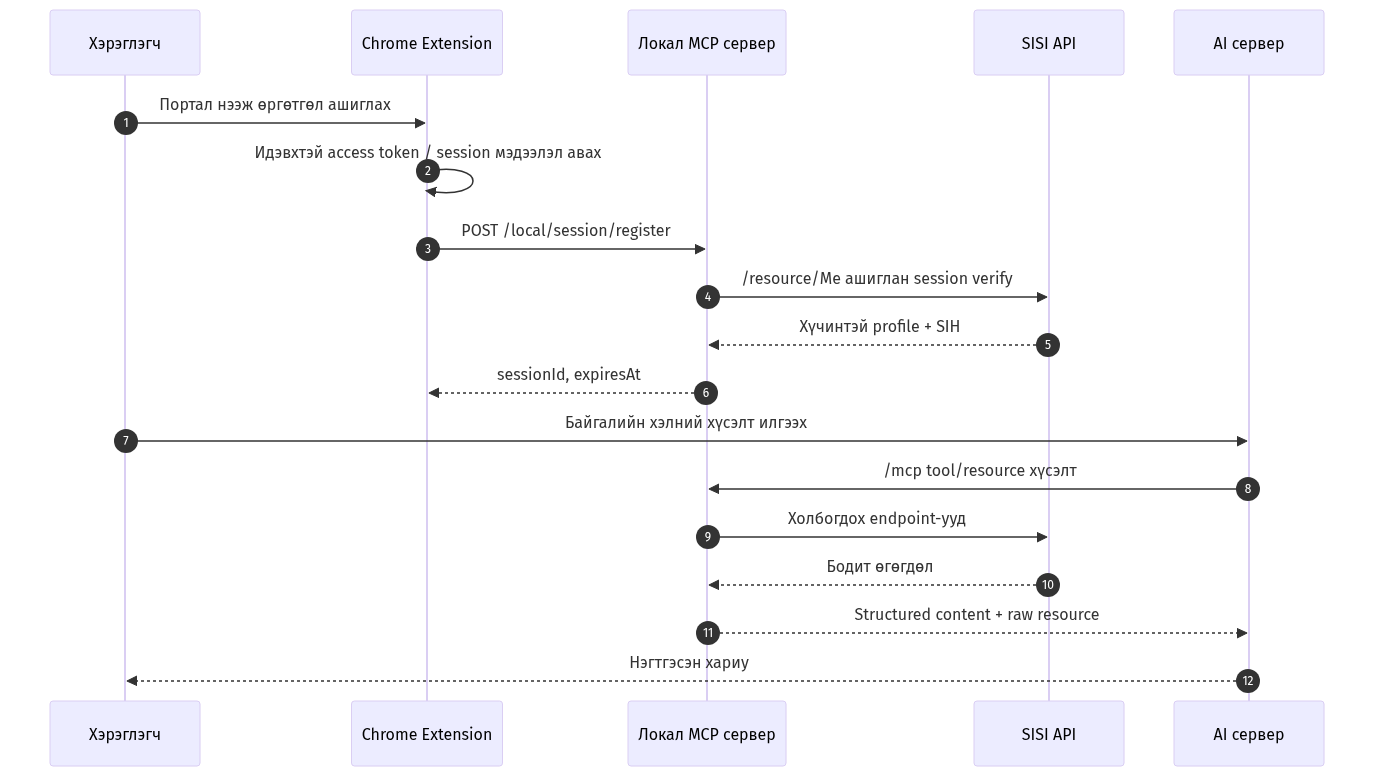
\includegraphics[width=\textwidth]{assets/diagrams/session-bootstrap.png}
  \caption{SISI сесс баталгаажуулалт ба MCP ашиглалтын урсгал}
  \label{fig:session-flow}
\end{figure}

Энэ шийдэл нь порталын access token болон cookie-г AI загварт шууд ил гаргахгүй, session idle TTL ашиглан локал сессийн насыг хязгаарлаж, хөтөчийн origin allowlist-аар зөвшөөрөгдсөн эх сурвалжаас л сесс бүртгэх боломжтой, мөн ижил механизмыг цаашдын багшийн портал болон бусад MCP интеграцын permission flow-д өргөтгөх боломжтой зэрэг шалтгаанаар хэрэгтэй.

\section{Домэйн төвтэй MCP загвар}

SISi системийн ухаалаг агентын интеграцын давхаргыг нэг том endpoint-оор бус, домэйнүүдээр салгасан. Одоогийн байдлаар дараах read-only домэйнүүд тодорхойлогдоод байна: Overview-д оюутны үндсэн мэдээлэл, нүүр хуудасны өгөгдөл, идэвхтэй хичээлүүд, Schedule-д хичээлийн болон шалгалтын хуваарь, Academic-д GPA, transcript, curriculum, request status, Financial-д төлбөр, үлдэгдэл, банкны мэдээлэл, Notifications-д аппын мэдэгдэл болон news, Student resources-д гарын авлага, баримт бичиг, картын мэдээлэл, Top menus/e-journal-д сонголтын туслах өгөгдөл, дүнгийн зарим нэгжүүд багтдаг.

Ийнхүү домэйнээр хуваасан нь дараа нь AI загварт ``ямар зорилгод ямар хэрэгсэл ашиглах вэ'' гэдгийг тогтмол дүрэмтэй болгоход тустай.

\section{Ирээдүйн өргөтгөлийн загвар}

Эцсийн зорилтот системд календарь, баримт бичиг, экспорт, мэдэгдэл зэрэг төрөл бүрийн гаднын үйлчилгээг MCP-ээр холбох ерөнхий MCP өргөтгөлүүд, багшийн API-г MCP хэлбэрт оруулж дүн оруулах зэрэг mutation workflow-г аюулгүй болгох багшийн порталын интеграц, мөн багш олон оюутны дүнг Excel файлаас уншуулан системд оруулах ажлыг хөнгөвчлөх Excel-д суурилсан ажиллагаа зэрэг өргөтгөлүүдийг шат дараатайгаар нэмэхээр төлөвлөж байна.

Эдгээрийг AI серверт хатуу кодлохын оронд тусдаа MCP server буюу MCP-compatible tool layer болгон оруулах нь архитектурын хувьд илүү оновчтой. Ингэснээр SISi системийн ухаалаг агент нь тодорхой нэг үйлчилгээтэй хэт холбогдсон хэрэгсэл бус, олон төрлийн системийг уялдуулах ерөнхий зохицуулагч давхарга болж хөгжинө.

\chapter{АШИГЛАХ ТЕХНОЛОГИ}

Энэхүү бүлэгт төслийн техникийн шийдлүүдийг сонгосон шалтгааныг тайлбарлана. Технологийн стек сонгохдоо дараах шалгуурыг баримталсан: нэг хэл дээр бүх давхаргыг хэрэгжүүлэх боломжтой байх, орчин үеийн AI tool-calling стандарттай нийцэх, мөн семестрийн хугацаанд практик хөгжүүлэлт хийх боломжтой байх.

\section{Хөгжүүлэлтийн хэл}

Төслийн бүх давхаргад TypeScript хэлийг ашиглах шийдлийг гаргасан. TypeScript нь JavaScript-ийн дээд багц бөгөөд статик төрлийн системийг (static type system) нэмж өгдөг. Төслийн хувьд TypeScript-ийн давуу тал нь Chrome extension болон MCP интеграцын хооронд ижил төрлийн тодорхойлолт (type definition) ашиглах боломжтой байдагт оршино. Жишээлбэл, MCP хэрэгслийн оролт гаралтын бүтцийг нэг удаа тодорхойлоод, AI сервер болон Chrome extension хоёуланд нь ашиглаж болно.

TypeScript нь хөгжүүлэлтийн явцад алдааг эрт илрүүлж, IDE-ийн автомат гүйцээлт (autocomplete) болон рефакторинг хийхэд тустай. Энэ нь ялангуяа олон модулиас бүрдсэн monorepo бүтэцтэй төсөлд чухал ач холбогдолтой юм.

\section{Model Context Protocol (MCP)}

Model Context Protocol SDK нь MCP стандартын албан ёсны TypeScript хэрэгжүүлэлт юм \cite{mcp-spec}. Энэхүү SDK нь MCP серверийг үүсгэж, tool, resource, prompt-уудыг бүртгэх боломж олгодог. Хэрэгслийн оролт гаралтын бүтцийг Zod schema ашиглан тодорхойлдог бөгөөд энэ нь runtime validation болон TypeScript type inference хоёуланг хангадаг. Тээврийн давхаргын хувьд stdio, HTTP, WebSocket зэрэг сонголтуудыг дэмждэг.

Одоогийн хэрэгжилтэд stdio transport ашиглан локал MCP сервер ажиллуулж байна. MCP серверийн хэрэгжилт нь төслийн гол техникийн бүрэлдэхүүн хэсэг бөгөөд SISI порталын API-тай холбогдох найман read-only хэрэгсэл тодорхойлогдсон.

\section{Chrome Extension}

Chrome extension хөгжүүлэхэд WXT framework ашиглаж байна \cite{wxt}. WXT нь орчин үеийн extension хөгжүүлэлтийн фреймворк бөгөөд уламжлалт extension хөгжүүлэлттэй харьцуулахад хэд хэдэн давуу талтай. Хөгжүүлэлтийн явцад Hot Module Replacement (HMR) ашиглан extension-ийг дахин ачаалахгүйгээр өөрчлөлтийг харах боломжтой. Extension-ийн бүх хэсэгт TypeScript ашиглах боломжтой бөгөөд шинэ Manifest V3 стандартыг бүрэн дэмждэг.

Extension-ийн хэрэглэгчийн интерфейсийг React ашиглан бүтээж байна. React нь компонент дээр суурилсан архитектур, виртуал DOM, өргөн хүрээний экосистем зэргээрээ extension UI хөгжүүлэхэд тохиромжтой. Popup доторх чат интерфейс нь хэрэглэгчийн үндсэн харилцааны цонх болж ажилладаг.

\section{AI интеграц}

AI загвартай ажиллахад Vercel AI SDK ашиглахаар төлөвлөж байна \cite{vercel-ai-sdk}. Энэ SDK нь хиймэл оюуны загваруудтай ажиллах TypeScript сан бөгөөд хэд хэдэн чухал боломжуудыг олгодог. Server-Sent Events ашиглан хэрэглэгчдэд бодит цагийн streaming хариу үзүүлэх боломжтой бөгөөд энэ нь урт хариулт үүсгэх үед хэрэглэгчийн туршлагыг сайжруулдаг. AI загварт хэрэгсэл тодорхойлж, загварын дуудлагыг автоматаар боловсруулах tool calling дэмжлэгтэй бөгөөд энэ нь MCP хэрэгслүүдтэй холбогдоход чухал. OpenAI, Anthropic, Google Gemini зэрэг үйлчилгээ үзүүлэгчдийг ижил интерфейсээр ашиглах боломжтой учраас ирээдүйд загвар солих уян хатан байдлыг хангадаг.

Прототип хөгжүүлэлтийн шатанд Google-ийн Gemini загварыг ашиглахаар төлөвлөж байна. Flash загвар нь хурдан хариу өгдөг бөгөөд прототип турших, хөгжүүлэлт хийхэд тохиромжтой. Gemini нь function calling-ийг сайн дэмждэг бөгөөд MCP хэрэгслүүдийг дуудахад ашиглах боломжтой. API дуудлагын өртөг харьцангуй бага учраас хөгжүүлэлтийн шатанд ашиглахад тохиромжтой. Эцсийн бүтээгдэхүүнд загварыг солих боломжтой бөгөөд Vercel AI SDK нь үүнийг хялбар болгодог.

\section{Monorepo бүтэц}

Төслийн кодын санг monorepo хэлбэрээр зохион байгуулсан. Monorepo нь олон апп, package-ийг нэг Git repository-д хадгалах арга бөгөөд код хуваалцах, хамаарлыг удирдахад тохиромжтой. Turborepo ашиглан monorepo-г удирдаж байгаа бөгөөд энэ нь build, test зэрэг даалгавруудын үр дүнг кэшлэж, хамааралгүй даалгавруудыг зэрэгцүүлэн ажиллуулдаг.

Одоогийн monorepo бүтэц нь apps болон packages гэсэн хоёр үндсэн хавтастай. Apps хавтаст extension (Chrome extension), server (AI сервер), web (туршилтын вэб интерфейс) багтдаг. Packages хавтаст mcp (MCP сервер), ui (дундын UI компонентууд), env (орчны тохиргоо) зэрэг дундын модулиуд багтдаг.

\section{Технологийн стекийн нэгдсэн хүснэгт}

Хүснэгт~\ref{tab:stack}--д төслийн технологийн стекийг нэгтгэн үзүүлэв.

\begin{table}[H]
  \centering
  \caption{Технологийн стек ба сонгосон шалтгаан}
  \label{tab:stack}
  \begin{tabularx}{\textwidth}{>{\raggedright\arraybackslash}p{3.3cm} >{\raggedright\arraybackslash}p{3.2cm} X}
    \toprule
    Ангилал & Технологи & Сонгосон шалтгаан \\
    \midrule
    Хэл & TypeScript & Extension, MCP интеграцын хооронд ижил type system ашиглах боломжтой \\
    MCP & Model Context Protocol SDK & Стандартчилсан tool, resource тодорхойлолт, Zod schema validation \\
    Extension & WXT + React & HMR, TypeScript дэмжлэг, Manifest V3, компонент архитектур \\
    AI давхарга & Vercel AI SDK & Streaming, tool calling, олон загварын дэмжлэг \\
    Загвар & Gemini & Хурдан хариу, tool calling дэмжлэг, бага өртөг \\
    Monorepo & Turborepo & Task caching, parallel execution, dependency graph \\
    \bottomrule
  \end{tabularx}
\end{table}

\section{Цаашид нэмэгдэх технологи}

Дараагийн шатанд хэд хэдэн технологийн хэсэг нэмэгдэх төлөвтэй байна. Гадаад MCP үйлчилгээнүүдтэй (Google Calendar, Notion гэх мэт) холбогдоход OAuth 2.0 зөвшөөрлийн урсгал шаардлагатай болно. Багшийн порталын Excel файлаас дүн оруулах workflow-д xlsx сан ашиглагдана. Mutation үйлдлүүдийг баталгаажуулах, хэрэглэгчээс зөвшөөрөл авах approval layer хэрэгжүүлэх шаардлагатай. Эдгээр өргөтгөл нь одоогийн суурь архитектуртай зөрчилдөхгүй, харин модульчлагдсан хэлбэрээр дээр нь нэмэгдэхээр төлөвлөсөн.

\chapter{ХЭРЭГЖҮҮЛЭЛТИЙН ЯВЦ БА ЦААШДЫН ТӨЛӨВЛӨГӨӨ}

\section{Одоогийн хэрэгжилтийн төлөв}

Энэхүү төслийг завсрын шатанд үнэлэхэд бүрэн бүтээгдэхүүн биш, харин ажиллаж эхэлсэн прототип гэж дүгнэх нь зөв. Хүснэгт~\ref{tab:progress}--д одоогийн төлөвийг нэгтгэн үзүүлэв.

\begin{table}[H]
  \centering
  \caption{Одоогийн хэрэгжилтийн төлөв}
  \label{tab:progress}
  \begin{tabularx}{\textwidth}{>{\raggedright\arraybackslash}p{4.6cm} >{\raggedright\arraybackslash}p{2.8cm} X}
    \toprule
    Ажлын хэсэг & Төлөв & Тайлбар \\
    \midrule
    Туршилтын вэб интерфейс & Хийсэн & Прототип турших зориулалттай суурь интерфейс бэлэн боловч эцсийн хэрэглээний үндсэн клиентээр төлөвлөөгүй \\
    AI серверийн суурь endpoint & Хийсэн & Elysia дээр `/ai` endpoint ажиллаж, загвараас стрийм хариу авч байна \\
    SISI MCP сервер & Хийсэн & Локал MCP сервер, health болон session bootstrap endpoint-уудтай \\
    Session баталгаажуулалт & Хийсэн & Cookie/header дээр тулгуурласан session verify, refresh, clear логик нэмэгдсэн \\
    Read-only MCP домэйнүүд & Хийсэн & Overview, schedule, academic, financial, notifications, resources, top menus, e-journal домэйнүүд тодорхойлогдсон \\
    AI ба MCP tool orchestration & Хийгдэж байгаа & AI серверийн message урсгал болон MCP хэрэгслийн бодит дуудагдалтыг нэгтгэх ажил үлдсэн \\
    Chrome extension-ийн интеграц & Хийгдэж байгаа & Extension-оор access token авч, дахин нэвтрэлтгүй session bootstrap хийх үндсэн урсгал боловсруулж байна \\
    Ерөнхий MCP өргөтгөлүүд & Төлөвлөсөн & Календарь, баримт бичиг, экспорт зэрэг төрөл бүрийн нэмэлт интеграц холбох боломжтой болгоно \\
    Багшийн порталын API интеграц & Төлөвлөсөн & Багшийн талын өгөгдөл болон mutation workflow-г MCP хэлбэрт оруулах \\
    Excel-ээс дүн оруулах урсгал & Төлөвлөсөн & Олон оюутны дүнг Excel файлаас системд оруулах ажиллагааг хөнгөвчлөх \\
    CSV export, mutation баталгаажуулалт & Төлөвлөсөн & Аюулгүй байдлын нэмэлт давхарга шаардлагатай \\
    Туршилт ба хэрэглэгчийн үнэлгээ & Төлөвлөсөн & Семестрийн сүүлчийн шатанд хийх \\
    \bottomrule
  \end{tabularx}
\end{table}

\section{Завсрын шатны гол үр дүн}

Одоогийн байдлаар дараах бодит ахиц гарсан. SISI API-д холбогдох MCP архитектурын эхний хувилбар ажиллаж эхэлсэн, оюутны өгөгдлийн хэд хэдэн чухал домэйныг read-only хэрэгсэл хэлбэрт оруулсан, туршилтын интерфейс, AI endpoint, Chrome extension-ийн суурь модуль бүрдсэн, цаашдын интеграцад ашиглах боломжтой модульчлагдсан monorepo бүтэц тогтсон, мөн хэрэгжсэн зүйл болон төлөвлөсөн зүйлсийг ялгаж баримтжуулах суурь бүрдсэн.

\section{Үлдсэн ажлууд}

Дараагийн шатанд AI серверээс MCP хэрэгслүүдийг бодитой дуудах orchestration урсгалыг нэгтгэх, хэрэглэгчийн зорилгоос хамаарсан tool routing болон confirmation flow загварчлах, Chrome extension-оос access token авч session reuse хийх урсгалыг тогтворжуулах, ерөнхий MCP өргөтгөлүүдийг турших, жишээ интеграцын оронд өргөтгөх архитектур бүрдүүлэх, багшийн порталын API-д холбогдох MCP давхаргыг төлөвлөх, Excel файлаас дүн оруулах workflow-г аюулгүй хэрэгжүүлэх шийдлийг загварчлах, CSV export, file output, audit trail логикийг тодорхойлох, мөн хэрэглэгчийн туршилт, жишиг сценари, үнэлгээний шалгуур боловсруулах зэрэг ажлуудыг тэргүүн ээлжид хийх шаардлагатай байна.

\section{Ажлын төлөвлөгөө}

\begin{table}[H]
  \centering
  \caption{Дараагийн шатны ажлын төлөвлөгөө}
  \label{tab:roadmap}
  \begin{tabularx}{\textwidth}{>{\raggedright\arraybackslash}p{3cm} >{\raggedright\arraybackslash}X}
    \toprule
    Хугацаа & Хийх ажил \\
    \midrule
    2026 оны 3-4 сар & AI серверийг MCP хэрэгслүүдтэй бүрэн уях, Chrome extension-ийн token reuse урсгалыг турших, use case-уудыг нарийвчлах \\
    2026 оны 4-5 сар & Ерөнхий MCP өргөтгөлийн загвар, mutation аюулгүй байдлын дүрэм, audit trail логикийг боловсруулах \\
    2026 оны 5 сар & Багшийн порталын API интеграц болон Excel-ээс дүн оруулах workflow-г турших, evaluation scenario бэлтгэх \\
    2026 оны 5-6 сар & Туршилт, хэрэглэгчийн үнэлгээ, алдаа засвар, төгсгөлийн тайлангийн өргөтгөл хийх \\
    \bottomrule
  \end{tabularx}
\end{table}

\section{Үнэлгээний анхны төлөвлөгөө}

Эцсийн шатанд системийг даалгавар амжилттай гүйцэтгэсэн хувь, хариу өгөх хугацаа, хэрэгслийн зөв сонголт, хэрэглэгчийн сэтгэл ханамж, мөн аюулгүй байдлын зөв хэрэгжилт гэсэн үндсэн хэмжүүрээр үнэлэхээр төлөвлөж байна. Өгөгдөл асуух, экспорт хийх, Excel-ээс дүн оруулах зэрэг use case бүр дээр амжилтын хувь, энгийн асуулт болон олон алхамт хүсэлтийн хариу өгөх хугацаа, AI ямар MCP хэрэгсэл ашигласан нь зөв эсэх, оюутнуудын богино асуулга, qualitative feedback, мөн mutation үйлдэл дээр баталгаажуулалт ажилласан эсэх зэргээр үнэлнэ.

Эдгээр хэмжүүр нь дипломын ажлын эцсийн шатанд зөвхөн техникийн demo бус, бодит хэрэглээний үнэ цэнийг нотлоход чухал үзүүлэлт болно.


\chapter*{ДҮГНЭЛТ}
\addcontentsline{toc}{chapter}{ДҮГНЭЛТ}
SISi системийн ухаалаг агент төсөл нь их сургуулийн дотоод порталын мэдээлэл болон цаашдын MCP интеграцуудыг байгалийн хэлний интерфейстэй холбох архитектурын чадамжийг завсрын хэрэгжилтээр баталгаажуулж байна. Судалгааны дүгнэлтээс үзэхэд энэ төрлийн системд зөвхөн хариу үүсгэдэг чатбот бус, бодит өгөгдөлтэй холбогдох найдвартай интерфейс, стандартчилсан хэрэгсэл, аюулгүй сессийн удирдлага, унших болон бичих үйлдлийг ялгасан зохиомж шаардлагатай байна.

Төслийн одоогийн шатанд хамгийн чухал ахиц нь SISI API-г MCP хэлбэрт оруулж, оюутны мэдээллийн хэд хэдэн үндсэн домэйнийг унших боломжтой болгосон явдал юм. Энэ нь цаашид дурын MCP интеграц нэмэх, олон алхамт команд гүйцэтгэх, экспорт болон баталгаажуулалт шаардсан үйлдлийг аюулгүй хэрэгжүүлэх, мөн багшийн порталын автоматжуулалтын урсгал нэмэх суурь болж өгнө.

Цаашдын ажлаар загварын tool-calling урсгалыг бүрэн холбох, Chrome extension-ийн access token суурьтай session bootstrap-ийг тогтворжуулах, шинэ MCP серверүүд болон багшийн порталын API-г нэгтгэх, mutation төрлийн үйлдлийн зөвшөөрлийн давхарга, туршилт болон хэрэглэгчийн үнэлгээг нэмэх замаар энэхүү төслийг төгсгөлийн шатанд бодит хэрэглээнд ойртсон дипломын систем болгон хөгжүүлнэ.

\cleardoublepage
\bibliographystyle{plainnat}
\bibliography{references}

\appendix
\chapter{АШИГЛАЛТЫН ХУВИЛБАРУУДЫН ДЭЛГЭРЭНГҮЙ ЖАГСААЛТ}

Энэ хавсралтад төслийн хүрээнд тодорхойлогдсон хэрэглэгчийн ашиглалтын хувилбаруудыг (use case) дэлгэрэнгүй тайлбарлана. Эдгээр нь системийн хөгжүүлэлт, туршилтын сценари боловсруулах үндэс болно. Хувилбар бүрийг тодорхойлохдоо хэрэглэгчийн хүсэлтийн жишээ, системийн хүлээгдэж буй хариу үйлдэл, шаардлагатай MCP хэрэгслүүд зэргийг тусгасан.

\section{Оюутны талын үндсэн хувилбарууд}

Эдгээр нь одоогийн MCP хэрэгслүүдээр дэмжигдэх боломжтой read-only хувилбарууд юм.

\subsection{Хуваарь харах}

\textbf{Хэрэглэгчийн хүсэлт:} ``Миний энэ долоо хоногийн хичээлийн хуваарийг харуулаач.''

\textbf{Системийн хариу үйлдэл:} Систем нь \texttt{get\_schedule} хэрэгслийг дуудаж, хэрэглэгчийн хичээлийн хуваарийг авна. Дараа нь өгөгдлийг боловсруулж, долоо хоногийн өдөр бүрээр ангилсан хуваарийг хэрэглэгчид ойлгомжтой хэлбэрээр харуулна. Хэрэв шалгалтын хуваарь байвал түүнийг тусад нь онцолж мэдээлнэ.

\textbf{Ашиглах MCP хэрэгсэл:} \texttt{get\_schedule}

\subsection{Дүн харах}

\textbf{Хэрэглэгчийн хүсэлт:} ``Миний өнгөрсөн семестрийн дүнг харуулаач. Голч хэд вэ?''

\textbf{Системийн хариу үйлдэл:} Систем нь \texttt{get\_academic\_record} хэрэгслийг дуудаж, хэрэглэгчийн академик бүртгэлийг авна. Өнгөрсөн семестрийн хичээлүүд, тэдгээрийн дүн, нийт голч (GPA) зэргийг тооцоолж харуулна. Хэрэв хэрэглэгч тодорхой хичээлийн талаар асуувал тухайн хичээлийн дүнг онцлон харуулна.

\textbf{Ашиглах MCP хэрэгсэл:} \texttt{get\_academic\_record}

\subsection{Төлбөрийн мэдээлэл}

\textbf{Хэрэглэгчийн хүсэлт:} ``Миний төлбөрийн үлдэгдэл хэд вэ? Хэзээ төлөх ёстой вэ?''

\textbf{Системийн хариу үйлдэл:} Систем нь \texttt{get\_financial\_overview} хэрэгслийг дуудаж, хэрэглэгчийн санхүүгийн мэдээллийг авна. Одоогийн үлдэгдэл, төлбөрийн хугацаа, өмнөх төлөлтүүдийн түүх зэргийг харуулна. Хэрэв төлбөрийн хугацаа ойрхон байвал анхааруулга өгнө.

\textbf{Ашиглах MCP хэрэгсэл:} \texttt{get\_financial\_overview}

\subsection{Мэдэгдэл харах}

\textbf{Хэрэглэгчийн хүсэлт:} ``Ямар нэгэн шинэ мэдэгдэл байна уу?''

\textbf{Системийн хариу үйлдэл:} Систем нь \texttt{get\_notifications} хэрэгслийг дуудаж, хэрэглэгчийн мэдэгдлүүдийг авна. Уншаагүй мэдэгдлүүдийг эхэлж харуулна. Мэдэгдлийн төрөл (захиргааны, хичээлийн, санхүүгийн гэх мэт)-өөр ангилж болно.

\textbf{Ашиглах MCP хэрэгсэл:} \texttt{get\_notifications}

\subsection{Ерөнхий мэдээлэл}

\textbf{Хэрэглэгчийн хүсэлт:} ``Миний оюутны мэдээллийг харуулаач.''

\textbf{Системийн хариу үйлдэл:} Систем нь \texttt{get\_student\_overview} хэрэгслийг дуудаж, хэрэглэгчийн ерөнхий мэдээллийг авна. Нэр, оюутны дугаар, мэргэжил, курс, статус зэргийг харуулна.

\textbf{Ашиглах MCP хэрэгсэл:} \texttt{get\_student\_overview}

\subsection{Олон мэдээлэл нэг дор}

\textbf{Хэрэглэгчийн хүсэлт:} ``Маргааш ямар хичээл байгаа, мөн дүнгийн мэдээлэл хэлээч.''

\textbf{Системийн хариу үйлдэл:} Систем нь хоёр хэрэгслийг дуудна: \texttt{get\_schedule} болон \texttt{get\_academic\_record}. Хоёр эх үүсвэрийн мэдээллийг нэгтгэж, маргаашийн хуваарь болон дүнгийн мэдээллийг хамтад нь харуулна.

\textbf{Ашиглах MCP хэрэгсэл:} \texttt{get\_schedule}, \texttt{get\_academic\_record}

\section{Өгөгдөл экспортлох хувилбарууд}

Эдгээр нь одоогийн MCP хэрэгслүүдийн гаралтыг файл хэлбэрт хөрвүүлэх хувилбарууд юм.

\subsection{Дүн CSV экспорт}

\textbf{Хэрэглэгчийн хүсэлт:} ``Миний бүх дүнг CSV файл болгож өгөөч.''

\textbf{Системийн хариу үйлдэл:} Систем нь \texttt{get\_academic\_record} хэрэгслийг дуудаж, бүх академик бүртгэлийг авна. Дараа нь өгөгдлийг CSV формат руу хөрвүүлж, хэрэглэгчид татаж авах боломж олгоно. CSV файлд хичээлийн нэр, кредит, дүн, семестр зэрэг багтана.

\textbf{Ашиглах MCP хэрэгсэл:} \texttt{get\_academic\_record}

\textbf{Тэмдэглэл:} Энэ нь read-only өгөгдөл дээр суурилсан хувиргалт бөгөөд mutation биш. AI загвар нь өгөгдлийг форматлах чадвартай.

\subsection{Хуваарь календарь руу}

\textbf{Хэрэглэгчийн хүсэлт:} ``Миний хичээлийн хуваарийг Google Calendar-т нэмж өгөөч.''

\textbf{Системийн хариу үйлдэл:} Систем нь \texttt{get\_schedule} хэрэгслийг дуудаж, хуваарийг авна. Дараа нь ерөнхий MCP өргөтгөлөөр (жишээ нь Google Calendar MCP) календарт event үүсгэнэ.

\textbf{Ашиглах MCP хэрэгсэл:} \texttt{get\_schedule}, Google Calendar MCP (төлөвлөсөн)

\textbf{Тэмдэглэл:} Энэ хувилбар нь ерөнхий MCP өргөтгөл шаарддаг бөгөөд дараагийн шатанд хэрэгжинэ.

\section{Ерөнхий MCP өргөтгөлийн хувилбарууд}

Эдгээр нь SISI-ийн өгөгдлийг гадаад системүүдтэй холбох хувилбарууд юм. Ирээдүйн хэрэгжилтэд багтана.

\subsection{Даалгавар reminder}

\textbf{Хэрэглэгчийн хүсэлт:} ``Миний даалгавруудын deadline-ийг reminder болгож тохируулаач.''

\textbf{Системийн хариу үйлдэл:} Систем нь SISI-ээс даалгаврын мэдээлэл авч, reminder MCP (жишээ нь Todoist, Notion) ашиглан хэрэглэгчийн сонгосон апп-д reminder үүсгэнэ.

\textbf{Ашиглах MCP хэрэгсэл:} SISI даалгавар хэрэгсэл, Reminder MCP (төлөвлөсөн)

\subsection{Тэмдэглэл хадгалах}

\textbf{Хэрэглэгчийн хүсэлт:} ``Энэ мэдээллийг Notion-д хадгалаач.''

\textbf{Системийн хариу үйлдэл:} Систем нь хэрэглэгчийн зааж өгсөн мэдээллийг Notion MCP ашиглан Notion database эсвэл page-д хадгална.

\textbf{Ашиглах MCP хэрэгсэл:} Notion MCP (төлөвлөсөн)

\section{Багшийн талын хувилбарууд}

Эдгээр нь багшийн порталтай холбогдсон хувилбарууд бөгөөд эцсийн дипломын ажилд хэрэгжинэ. Mutation үйлдэл агуулдаг тул аюулгүй байдлын нэмэлт шаардлагатай.

\subsection{Excel-ээс дүн оруулах}

\textbf{Хэрэглэгчийн хүсэлт:} ``Энэ Excel файлаас оюутнуудын дүнг системд оруулаач.''

\textbf{Системийн хариу үйлдэл:} Систем нь дараах алхмуудыг гүйцэтгэнэ. Эхлээд Excel файлыг уншиж, мөр бүрийн өгөгдлийг задлана. Дараа нь мөр бүрийг шалгана: оюутны код зөв эсэх, дүн зөвшөөрөгдсөн хүрээнд байгаа эсэх, хичээлийн код таарч байгаа эсэх. Алдаатай мөрүүдийг жагсааж, багшид харуулна. Багш баталгаажуулсны дараа зөв мөрүүдийг системд оруулна. Эцэст нь үр дүнгийн тайлан гаргана: амжилттай оруулсан, алдаатай, алгассан мөрүүдийн тоо.

\textbf{Ашиглах MCP хэрэгсэл:} Багшийн портал MCP (төлөвлөсөн), Excel parsing

\textbf{Аюулгүй байдал:} Энэ нь mutation үйлдэл тул хэд хэдэн хамгаалалт шаардлагатай. Оруулахын өмнө бүх өгөгдлийг багшид харуулж баталгаажуулалт авах шаардлагатай. Мөр бүрийн validation хийх хэрэгтэй. Audit trail бичих буюу хэн, хэзээ, ямар өгөгдөл оруулсныг бүртгэх шаардлагатай. Rollback буюу буцаах боломжтой байх хэрэгтэй.

\subsection{Дүнгийн тайлан}

\textbf{Хэрэглэгчийн хүсэлт:} ``Миний ангийн дүнгийн тархалтыг харуулаач.''

\textbf{Системийн хариу үйлдэл:} Систем нь багшийн порталаас ангийн дүнгийн өгөгдлийг авч, статистик тооцоолно: дундаж, медиан, дээд/доод дүн, дүнгийн тархалт (histogram). Энэ мэдээллийг багшид ойлгомжтой хэлбэрээр харуулна.

\textbf{Ашиглах MCP хэрэгсэл:} Багшийн портал MCP (төлөвлөсөн)

\section{Нарийвчилсан харилцааны хувилбарууд}

Эдгээр нь хэрэглэгчийн асуултад илүү нарийвчилсан хариу шаардах хувилбарууд юм.

\subsection{Хичээл санал болгох}

\textbf{Хэрэглэгчийн хүсэлт:} ``Дараагийн семестрт ямар хичээл үзэх боломжтой вэ? Урьдчилсан шаардлагыг хангасан хичээлүүдийг харуулаач.''

\textbf{Системийн хариу үйлдэл:} Систем нь \texttt{get\_academic\_record} болон хичээлийн мэдээллийн хэрэгслийг ашиглан хэрэглэгчийн үзсэн хичээлүүд, тэдгээрийн дүнг авна. Дараа нь урьдчилсан шаардлагын (prerequisite) логикоор үзэх боломжтой хичээлүүдийг тооцоолж санал болгоно.

\textbf{Ашиглах MCP хэрэгсэл:} \texttt{get\_academic\_record}, хичээлийн каталог хэрэгсэл (төлөвлөсөн)

\subsection{Төгсөлтийн шаардлага}

\textbf{Хэрэглэгчийн хүсэлт:} ``Төгсөхөд хэдэн кредит дутуу байна вэ? Ямар хичээл заавал үзэх ёстой вэ?''

\textbf{Системийн хариу үйлдэл:} Систем нь хэрэглэгчийн академик бүртгэл болон мэргэжлийн төгсөлтийн шаардлагыг харьцуулж, дутуу кредит, заавал үзэх хичээлүүдийг тооцоолно.

\textbf{Ашиглах MCP хэрэгсэл:} \texttt{get\_academic\_record}, \texttt{get\_student\_overview}, төгсөлтийн шаардлагын хэрэгсэл (төлөвлөсөн)

\section{Тэмдэглэл}

Дээрх use case-уудаас зарим нь одоогийн хэрэгжилтээр дэмжигдэж байгаа бол зарим нь дараагийн шатны ажлуудтай холбоотой.

Одоо боломжтой хувилбарууд нь хуваарь харах, дүн харах, төлбөрийн мэдээлэл, мэдэгдэл харах, ерөнхий мэдээлэл, олон мэдээлэл нэг дор, CSV экспорт (AI форматлалт) зэрэг юм.

Дараагийн шатанд хэрэгжих хувилбарууд нь ерөнхий MCP өргөтгөлүүд (календарь, Notion), хичээл санал болгох, төгсөлтийн шаардлага зэрэг юм.

Эцсийн дипломд хэрэгжих хувилбарууд нь багшийн порталын бүх хувилбарууд, Excel дүн оруулах, mutation баталгаажуулалт зэрэг юм.

Туршилтын шатанд эдгээр use case-уудыг ашиглан системийн амжилтын хувь, хариу өгөх хугацаа, хэрэглэгчийн сэтгэл ханамж зэргийг хэмжинэ.

\chapter*{МЭРГЭЖЛИЙН НЭР ТОМЬЁОНЫ ТАЙЛБАР}
\addcontentsline{toc}{chapter}{Мэргэжлийн нэр томьёоны тайлбар}

\begin{table}[H]
  \centering
  \caption{Мэргэжлийн нэр томьёо}
  \label{tab:glossary}
  \begin{tabularx}{\textwidth}{>{\raggedright\arraybackslash}p{4.5cm} X}
    \toprule
    Нэр томьёо & Товч тайлбар \\
    \midrule
    SISi системийн ухаалаг агент (SISi Intelligent Agent) & SISI порталд суурилсан хиймэл оюуны туслах систем. Хэрэглэгчийн байгалийн хэлний хүсэлтийг бодит системийн үйлдэл болгон хувиргах зориулалттай. \\
    \addlinespace
    Model Context Protocol (MCP) & Хиймэл оюуны загварт гадаад хэрэгсэл, өгөгдлийн эх үүсвэрийг стандартчилсан аргаар холбох нээлттэй протокол. tool, resource, prompt гэсэн үндсэн нэгжүүд ашиглана. \\
    \addlinespace
    AI Agent (Хиймэл оюуны агент) & Хэлний загвар, орчны өгөгдөл, хэрэгслүүд, үйлдлийн урсгалыг нэгтгэсэн ухаалаг систем. Зөвхөн хариу үүсгэх бус, бодит үйлдэл гүйцэтгэх чадвартай. \\
    \addlinespace
    Tool-calling & Хиймэл оюун бодит системтэй харилцахдаа хэрэгслүүдийг дуудаж, өгөгдөл авах, үйлдэл гүйцэтгэх механизм. \\
    \addlinespace
    MCP Server & Model Context Protocol-ийн стандартад нийцсэн сервер. Гаднын системүүдийг (SISI портал, календарь, баримт бичиг гэх мэт) хиймэл оюунтай холбох давхарга. \\
    \addlinespace
    Session Bootstrap & Хэрэглэгчийг дахин нэвтрүүлэхгүйгээр одоогийн access token, cookie ашиглан сесс үүсгэх механизм. \\
    \addlinespace
    Access Token & Хэрэглэгчийн системд нэвтэрснийг баталгаажуулж, API хүсэлтийг зөвшөөрөх нууцлалын түлхүүр. \\
    \addlinespace
    Read-only Tool & Өгөгдөл унших, харах зориулалттай MCP хэрэгсэл. Mutation үйлдэл хийх боломжгүй. \\
    \addlinespace
    Mutation & Өгөгдөл бичих, өөрчлөх, устгах зэрэг системд өөрчлөлт оруулах үйлдэл. Баталгаажуулалт шаарддаг. \\
    \addlinespace
    Chrome Extension & Вэб хөтөчид нэмэлт функц нэмэх програм. Энэхүү төслөөр порталын сессийг авах, хэрэглэгчийн интерфейс харуулахад ашиглана. \\
    \addlinespace
    Tool Orchestration & Олон хэрэгслийг дарааллан эсвэл параллелаар дуудаж, үр дүнг нэгтгэх үйл явц. \\
    \addlinespace
    Domain & Системийн тодорлхой чиглэл (хуваарь, дүн, санхүү гэх мэт). \\
    \addlinespace
    Prompt & Хиймэл оюуны загварт өгөх заавар, асуулт, эсвэл контекст. \\
    \addlinespace
    Orchestration Layer & AI сервер дээр хэрэгслүүдийг дуудах, хариулт үүсгэх үйл явцыг удирдах модуль. \\
    \addlinespace
    Audit Trail & Mutation үйлдлүүдийн түүх, лог бичлэг. Аюулгүй байдал, хяналтын зориулалттай. \\
    \addlinespace
    Confirmation Flow & Эрсдэлтэй үйлдэл хийхээс өмнө хэрэглэгчээс дахин баталгаа авах механизм. \\
    \addlinespace
    Workflow & Олон алхамт үйлдлүүдийн дараалал. Жишээ нь: Excel файлаас дүн оруулах. \\
    \addlinespace
    API (Application Programming Interface) & Системүүд хоорондоо өгөгдөл солилцох протокол. \\
    \addlinespace
    Elysia & TypeScript хэл дээр бичигдсэн хөнгөн жинтэй вэб фреймворк. \\
    \addlinespace
    React & Хэрэглэгчийн интерфейс бүтээхэд ашиглах frontend сан. \\
    \addlinespace
    Bun & JavaScript/TypeScript код ажиллуулах шинэ runtime. Хурдан, хөнгөн. \\
    \addlinespace
    Turborepo & Monorepo удирдах хэрэгсэл. Олон апп, package-ийг нэг кодын сангаас зохицуулна. \\
    \addlinespace
    Drizzle ORM & TypeScript-д зориулсан өгөгдлийн сантай харилцах сан. \\
    \bottomrule
  \end{tabularx}
\end{table}

\vspace{1cm}
\noindent\textbf{Тэмдэглэл:} Энэхүү тайландаа анх удаа гарч буй мэргэжлийн нэр томьёог товч тайлбартай хамт оруулсан. Давтагдах үед хэвээрээ англи нэр томьёог ашиглана.


\end{document}
